\documentclass[text07.tex]{subfiles}
\begin{document}
%
% Chapter 6
% 
\chapter{WEBページの仕組みを知ろう}

% 
% section 6.1
% 
\section{今回の授業}

% 
% subsection 6.1.1
% 
\subsection{目標と\ruby{授業内容}{じゅぎょうないよう}}

\begin{itemize}
	\item ネチケットを知ろう
	\item ネットワークについて学ぼう
	\item CGIを使いこなそう
\end{itemize}

\subsection*{注意点}
\begin{itemize}
	\item 授業の合間の\ruby{休憩}{きゅうけい}では、遠くのものを\ruby{眺}{なが}めたりして目を休めましょう。
	\item 水分\ruby{補給}{ほきゅう}をこまめにしましょう。
	\item 先生が説明中は先生の話を聞きましょう。
	\item わからないことがあったらTAの先生方にすぐ聞きましょう。
\end{itemize}

\subsection*{教科書について}
\begin{itemize}

	\item 教科書では、\ruby{具体的}{ぐたいてき}な操作の手順が説明され、それを\ruby{応用}{おうよう}した問題があります。\\
		  まずは、説明をよく読みながら試してみましょう。\\
		  そのあと問題をと解きましょう。
	\item 問題をクリアしたらシールラリーカードにスタンプを押しましょう。

	\item すべての問題をクリアできたらTAの先生にラリーカードを見せて、\\
	      Complete(コンプリート)スタンプをもらいましょう。
	\item 授業中に終わらなかった問題は、できるだけ家でやって終わらせましょう。
	\item 授業中にわからないところがあったらすぐにTAの先生に聞きましょう。

	\item 家でわからないことがあったら、すぐに\ruby{質問}{しつもん}フォームから\ruby{質問}{しつもん}しましょう。
\end{itemize}

\subsection*{教材を自分のフォルダに置く}
\begin{itemize}
	\item /usr/local/share/ome にあるフォルダ 07 をホームディレクトリにコピーしましょう。
	\item やり方を忘れてしまった人は、「第 1 回 1.4.1. 教材を準備しよう」を参考にしてみてください。

\end{itemize}

\clearpage

\subsection*{\bfseries ネチケット}
% \refstepcounter{PagePtr}\label{P:Netiquette}

学校の先生たちから、「友達を\ruby{傷}{きず}つけてはいけない」、「\ruby{敬語}{けいご}は正しく使おう」、などとマナーを教えられてきたと思います。
マナーは、ネットワークにも\ruby{存在}{そんざい}します。ネットワークのマナーを「\textbf{ネチケット}」と言います。
ネットをするときに、何も考えずに利用していると気がつかずに問題や\ruby{犯罪}{はんざい}に手を\ruby{染}{そ}める\ruby{可能性}{かのうせい}があります。
他人に\ruby{迷惑}{めいわく}をかけないことに加えて、ネチケットを守らない人から自分を守るために理解をしましょう。

\begin{description}

	\item [\ruby{誰}{だれ}かが作ったものを勝手に使わない]~\\
	\begin{minipage}[b]{0.65\textwidth}
		インターネットをしているとたくさんの\ruby{画像}{がぞう}や文章などのデータがあります。見て楽しむ\ruby{程度}{ていど}には問題ないですが、誰かが作ったものや\ruby{情報}{じょうほう}には\ruby{著作権}{ちょさくけん}というものがあります。\ruby{法律}{ほうりつ}で勝手に使うことは\ruby{禁止}{きんし}されているから気をつけましょう。ただし、\ruby{著作権}{ちょさくけん}は\ruby{個人}{こじん}で楽しむもの、\ruby{出典}{しゅってん}を明らかにして、引用することは\ruby{認}{みと}められています。
	\end{minipage}\hfill
	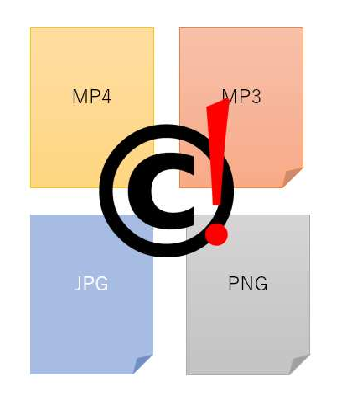
\includegraphics[width=0.2\textwidth]{../../asset/image/ome7-img001}
	\item [人を傷つけることや、迷惑になることはやめる]~\\
		  インターネットは自分以外の人も使っています。だから、自分勝手なことや悪い言葉を使ってばかりいると人を傷つけたり、\ruby{不快}{ふかい}に思われて犯罪に\ruby{巻}{ま}き\ruby{込}{こ}まれたり、\ruby{訴}{うった}えられたりする可能性もあります。清らかに生きていきましょう。
	\item [他のひとたちが\ruby{困}{こま}らない文字情報を使う]~\\
		  ネットワークを使っている人たちはみんな同じものを使っているとは限りません。
		  使っている機種が、PCだったり、スマートフォンだったり、ラズベリーパイだったりします。機種によっては、絵文字や特殊文字が見えなくなることが考えられます。
	\item [迷惑メールは見ない、送らない]~\\
		  悪い人が色々な都合で出してくる\ruby{怪}{あや}しいメールのことです。。これには、変なアドレスがはられてい
		  たり、知らないソフトウェアが貼り付けられたりすることがあります。それを見るとウイルスという悪いものが入ってくることことがあります。ウイルスはコンピュータが\ruby{壊}{こわ}れたり、\ruby{操作}{そうさ}出来なくなったりするものもあります。犯罪者の協力をしたと思われることもあるので、怪しいメールは\ruby{絶対}{ぜったい}に開かないようにしましょう。また、チェーンメール（\ruby{呪}{のろ}いのメールなど）は絶対に信じず他の人に送ってはいけません。メール本文中に、『誰かに回して』 『○○人に転送するように』などと書かれているメールを受け取ったのなら、それはどんな内容でもチェーンメールです。
	\item [自分の情報を外に\ruby{漏}{も}らさない]~\\
		  自分の名前や、住所などをネットにあげるのはとても\ruby{危}{あぶ}ないから止めましょう。悪い人の目に入ってしまうと家族の身の\ruby{危険}{きけん}にもつながり命の\ruby{保証}{ほしょう}ができません。また、ネットに一度でもあげてしまうと消すことができなくなります。多くの人の目につくからデータが広がってしまうこともあります。ネットにデータをあげるときは問題が無いか\ruby{確認}{かくにん}してからあげましょう。
\end{description}

% \clearpage

% \subsection*{教材を自分のフォルダに置こう}
% まずは、今回利用する教材をコピーしましょう。
% これまでと同じように、/usr/local/share/ome という場所にあるフォルダ 07をコピーして、/home/ユーザー名 に貼り付けてください。

% やり方を忘れてしまった人は、「第1回 4.1 例題1-18 教材をじぶんのフォルダに置こう」 を参考にしてみてください。

\clearpage\end{document}
